\documentclass[10pt,twocolumn,letterpaper]{article}

\usepackage{cvpr}
\usepackage{times}
\usepackage{epsfig}
\usepackage{graphicx}
\usepackage{amsmath}
\usepackage{amssymb}
\usepackage{booktabs}

% Include other packages here, before hyperref.

% If you comment hyperref and then uncomment it, you should delete
% egpaper.aux before re-running latex.  (Or just hit 'q' on the first latex
% run, let it finish, and you should be clear).
\usepackage[breaklinks=true,bookmarks=false]{hyperref}

\cvprfinalcopy % *** Uncomment this line for the final submission

\def\cvprPaperID{****} % *** Enter the CVPR Paper ID here
\def\httilde{\mbox{\tt\raisebox{-.5ex}{\symbol{126}}}}

% Pages are numbered in submission mode, and unnumbered in camera-ready
%\ifcvprfinal\pagestyle{empty}\fi
\setcounter{page}{1}
\begin{document}

%%%%%%%%% TITLE

\title{Modelling and Functional Characterization of the Pyridoxamine Kinase/Phosphomethylpyrimidine Kinase Domain Family}

\author{
Marco Uderzo\\
{\small Department of Mathematics, University of Padua}\\
{\tt\small marco.uderzo@studenti.unipd.it}\\
{\tt\small ID: 2096998} \\
\and
Tanner Graves\\
{\small Department of Mathematics, University of Padua}\\
{\tt\small tanneraaron.graves@studenti.unipd.it}\\
{\tt\small ID: 2073559} \\
\and
Claudio Palmeri \\
{\small Department of Mathematics, University of Padua}\\
{\tt\small claudio.palmeri@studenti.unipd.it}\\
{\tt\small ID: 2062671} \\
}


\maketitle
%\thispagestyle{empty}


%%%%%%%%% ABSTRACT
\begin{abstract}
    This project aims to build a sequence model and provide a comprehensive functional characterization of the Pyridoxamine Kinase/Phosphomethylpyrimidine Kinase domain family. The models' accuracy is benchmarked against Pfam annotations in the SwissProt database. Furthermore, we delved into the functional and structural properties of the domain family, analyzing the taxonomic lineage, assessing Gene Ontology (GO) annotations for functional enrichment, and searching for significantly conserved short motifs inside the family. (Include findings in the abstract)
\end{abstract}

%%%%%%%%% BODY TEXT
\section{Introduction}

\subsection{Protein Domains}

A protein domain represents a conserved part of a protein's sequence and three-dimensional structure, capable of evolving, functioning, and existing independently from the rest of the protein chain. These domains, each forming a stable and compact three-dimensional structure, are essential components in proteins, often occurring in various combinations across different proteins. Domains are fundamental in molecular evolution, serving as versatile building blocks that can be rearranged to form proteins with diverse functions. This adaptability and independence make them crucial in understanding protein structure and function.

\subsection{Pyridoxamine Kinase / Phosphomethylpyrimidine Kinase}

Pyridoxamine Kinase/Phosphomethylpyrimidine Kinase family is a group of enzymes that play key roles in various biochemical pathways, particularly in the metabolism of vitamins and coenzymes. This family includes two distinct but related enzymes:

\begin{itemize}
\item \textbf{Pyridoxamine Kinase}: This enzyme is involved in the vitamin B6 metabolism pathway. Vitamin B6 exists in different forms, including pyridoxamine, pyridoxal, and pyridoxine. Pyridoxamine kinase specifically catalyzes the phosphorylation of pyridoxamine, converting it into pyridoxamine 5'-phosphate. This is an important step in the salvage pathway of vitamin B6, which is crucial for its recycling and maintenance within the cell.

\item \textbf{Phosphomethylpyrimidine Kinase}: This enzyme plays a role in the biosynthesis of thiamine (vitamin B1), which is essential for numerous cellular functions, particularly in carbohydrate metabolism.
\end{itemize}

Both these enzymes, due to their roles in vitamin metabolism, are crucial for maintaining cellular health and function. Disruptions in these pathways can lead to vitamin deficiencies, affecting numerous biological processes.

\subsection{Objective of the Study}

This project aims to build a sequence model and provide a comprehensive functional characterization of the Pyridoxamine Kinase/Phosphomethylpyrimidine Kinase domain family. (Write a small preamble of the goals of this project, even if it is similar to what is written in the abstract).

\section{Methods and Results}

\subsection{Model Building}

Firstly, we investigated the target family to model - Pyridoxamine Kinase/Phosphomethylpyrimidine Kinase - and verified that the provided representative \texttt{A0A0J9X285} protein sequence, having Pfam domain \texttt{PF08543}, is indeed characteristic of the protein family. 
This was done by retrieving the seed alignment used to generate the HMM defining the Pfam family from \textit{InterPro}, and aligning the representative query sequence to the seed alignment using \textit{JalView}.

The query spans the length of the seed alignment and the gaps opened in the query correspond to low occupancy regions in the seed alignment. This bolsters our confidence that performing a homology search with our query sequence will be able to return sequences belonging to the \texttt{PF08543} family. This was done by performing a Position-Specific Iterated BLAST (\texit{PSI-BLAST}) search on \textit{SwissProt}. The results were downloaded as a \texttt{.fasta} file and opened in \textit{JalView}, where we added our query sequence as a reference. The FASTA file was aligned with the query sequences using \textit{Clustal Omega}.

The query sequence overlapped the primary conserved regions of the MSA, and the majority of positions outside of the query had very low occupancy, consisting of sequences that were unusually long. The query bounds for the MSA are observed to be reasonable bounds to trim the MSA, so positions outside this range were trimmed from it. \\

Sequences that opened gaps more than a couple residues long were investigated by referencing the BLAST hit corresponding to that sequence. Many of these instances were from Eukariotes - which is atypical for this family - and were of reasonable quality. Since it is useful to include this information, no sequences reported by BLAST were discarded. \\

The MSA was finalized by removing the query sequence, and it was then processed to generate a \textit{Position-Specific Scoring Matrix (PSSM)} using the command line \texttt{PSI-BLAST} tool, with the SwissProt database as the reference. Finally, the HMM was build using the \texttt{hmmer hmmbuild} command.

\subsection{Model Evaluation}

The PSSM predictions were generated through PSI-BLAST searches against the SwissProt database.
Parallelly, HMM searches were conducted, the results of which were parsed to extract alignments between the HMM and sequences in the SwissProt database.

\subsubsection{PSSM Protein-Level Performance Evaluation}

The protein-level performances of the PSSM model are shown in the table below:

\begin{center}
    \begin{tabular}{lc}
        \toprule
        Metric & Value \\
        \midrule
        Precision & 0.894 \\
        Recall & 0.227 \\
        F1-Score & 0.361 \\
        Balanced Accuracy & 0.613 \\
        MCC & 0.45 \\
        \bottomrule
    \end{tabular}
\end{center} 

\begin{center}
    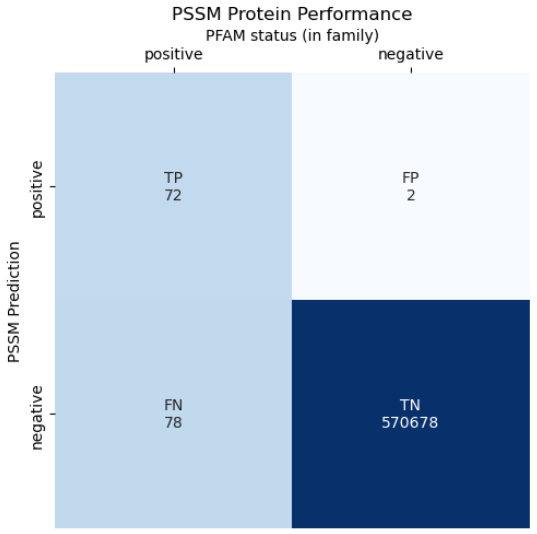
\includegraphics[scale=0.45]{report/img/pssm_prot_performance.png}
\end{center}

\subsubsection{PSSM Residue-Level Performance Evaluation}

The residue-level performances of the PSSM model are shown in the table below:


\begin{center}
    \begin{tabular}{lc}
        \toprule
        Metric & Value \\
        \midrule
        Precision & 0.91 \\
        Recall & 0.28 \\
        F1-Score & 0.429 \\
        Balanced Accuracy & 0.64 \\
        MCC & 0.505 \\
        \bottomrule
    \end{tabular}
\end{center} 

\begin{center}
    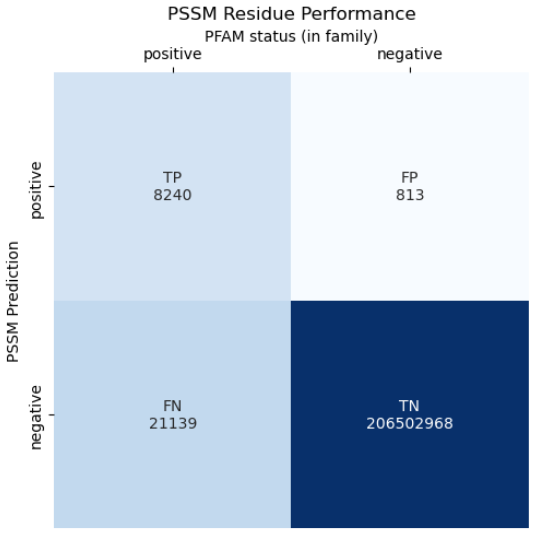
\includegraphics[scale=0.45]{report/img/pssm_res_performance.png}
\end{center}

\subsubsection{HMM Protein-Level Performance Evaluation}


The protein-level performances of the HMM model are shown in the table below:

\begin{center}
    \begin{tabular}{lc}
        \toprule
        Metric & Value \\
        \midrule
        Precision & 0.993 \\
        Recall & 0.993 \\
        F1-Score & 0.993 \\
        Balanced Accuracy & 0.996 \\
        MCC & 0.993 \\
        \bottomrule
    \end{tabular}
\end{center} 

\begin{center}
    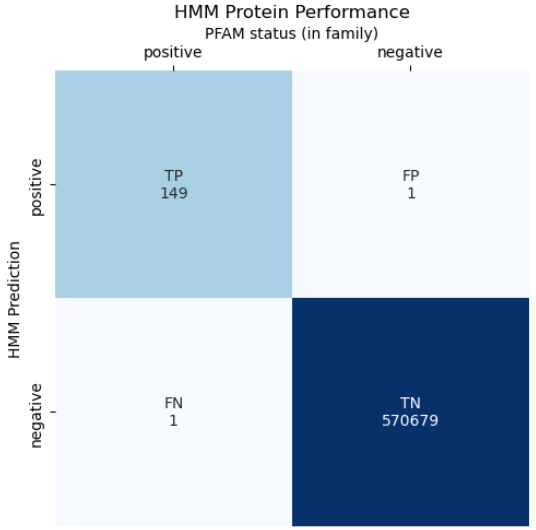
\includegraphics[scale=0.45]{report/img/hmm_prot_performance.png}
\end{center}

\subsubsection{HMM Residue-Level Performance Evaluation}

The residue-level performances of the HMM model are shown in the table below:

\begin{center}
    \begin{tabular}{lc}
        \toprule
        Metric & Value \\
        \midrule
        Precision & 0.989 \\
        Recall & 0.974 \\
        F1-Score & 0.982 \\
        Balanced Accuracy & 0.987 \\
        MCC & 0.982 \\
        \bottomrule
    \end{tabular}
\end{center} 

\begin{center}
    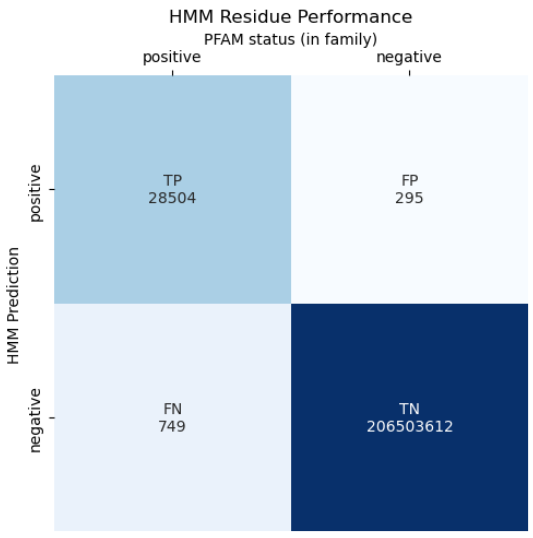
\includegraphics[scale=0.45]{report/img/hmm_res_performance.png}
\end{center}

As indicated by the confusion matrix, the HMM predictions match the target PFAM family very closely.

\subsection{Taxonomy}

To construct the taxonomic tree, we assembled the lineage data derived from the \textit{SwissProt} database, corresponding to the protein family under investigation. The lineages were used to generate a comprehensive taxonomic hierarchy, which was enriched with node-specific information, including taxonomic names and the frequency of each taxon's occurrence within our data. In our tree, the size of each node indicates how many examples (or leaves) have that taxonomy term. This provides a good visualization of the lineage of taxonomy terms characteristic of our family (i.e. Bacteria, Pseudomonadota, Gammaproteobacteria, Enterobacterales, Enterobacteriaceae, E. coli).

The taxonomic tree is shown below. In order to view it in full resolution, we refer to the corresponding \hyperref[sec:taxtree]{section} in the appendix, or directly to the \texttt{TaxonomyTree.pdf} file that can be found in the supplementary material.

\begin{center}
    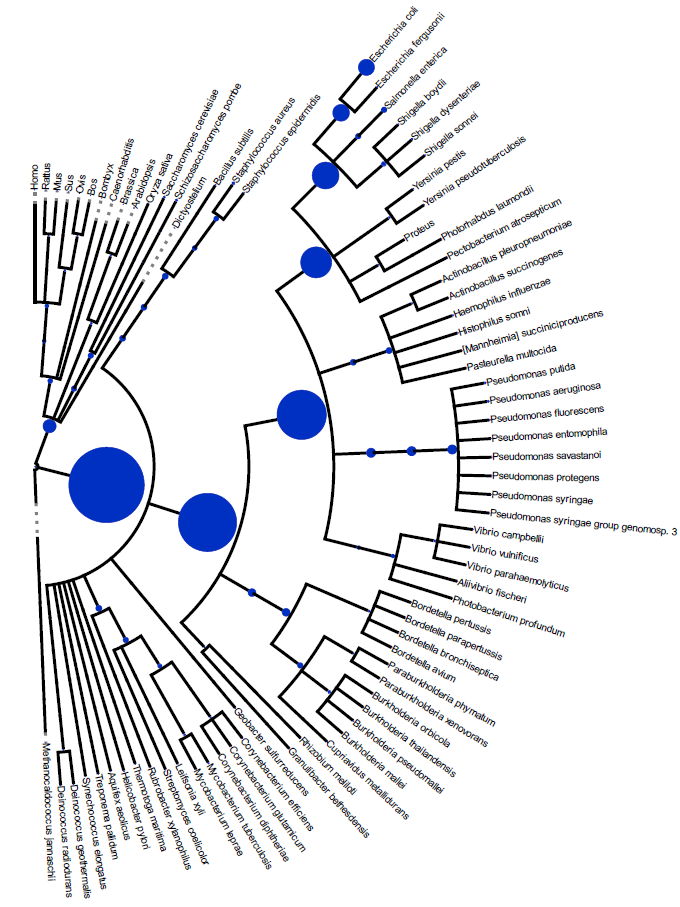
\includegraphics[scale=0.4]{report/img/taxonomy_tree.png}
\end{center}

\subsection{Functional Enrichment with Gene Ontology Annotation}

We performed Functional Enrichment Analysis using \textit{Gene Ontology} (GO) annotations by extracting the \textit{molecular function}, \textit{cellular component}, and \textit{biological process} data.

In order to visualize which GO Terms are characteristic of our family, we can plot the enrichment (probability) of observing a GO Term over both our model family and the totality of \textit{SwissProt}. Selecting the terms with the highest odds, or the ratio of probability that the term is observed in the family and all of \textit{SwissProt} gives us clues about which terms are most characteristic. 

\begin{center}
    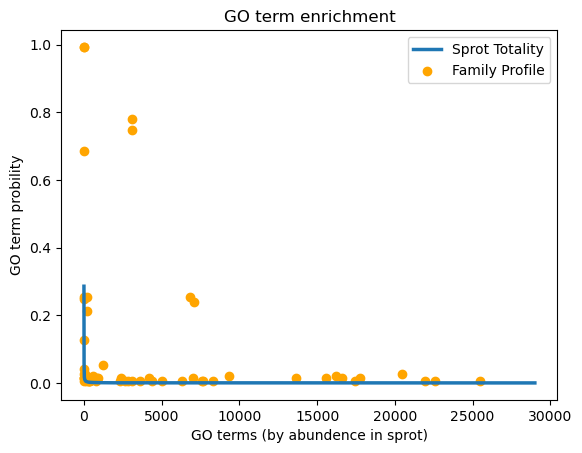
\includegraphics[scale=0.4]{report/img/go_term_enrichment.png}
\end{center}

\begin{center}
    \begin{tabular}{lcc}
        \toprule
        GO Term ID & Term Name & Odds \\
        \midrule
        GO:0042817	& \small{pyridoxal metabolic process} &	3805.53 \\
        GO:0008478	& \small{pyridoxal kinase activity} &	3773.28 \\
        GO:0009443	& \small{pyridoxal 5'-phosphate salvage} &	3642.90 \\
        GO:0008972	& \small{phosphomethylpyrim. kin. act.} &	3615.25 \\
        GO:0008902	& \small{hydroxymethylpyrim. kin. act.} &	3605.24 \\
        GO:0009230	& \small{thiamine catabolic process} &	1902.76 \\
        GO:0042818	& \small{pyridoxamine metabolic process} &	1427.07\\
        GO:0042816	& \small{vitamin B6 metabolic process} &	1268.51\\
        GO:0010054	& \small{trichoblast differentiation} &	1268.51 \\
        GO:0036172	& \small{thiamine salvage} &	1087.29 \\
        GO:0042822	& \small{pyridoxal phosphate metab. proc.} &	951.38 \\
        GO:0070280	& \small{pyridoxal binding} &	845.67 \\
        GO:0031403	& \small{lithium ion binding} &	634.25 \\
        GO:0042819	& \small{vitamin B6 biosynthetic proc.} &	543.64 \\
        GO:0050334	& \small{thiaminase activity} &	456.66 \\
        GO:0097159	& \small{organic cyclic compound binding} &	200.29 \\
        GO:0008614	& \small{pyridoxine metabolic process} &	131.22 \\
        \bottomrule
    \end{tabular}
\end{center} 
\begin{center}
    \small{Most characteristic GO Terms}
\end{center}



By using Fisher's Exact Test, we realized that the p-value is extremely close to zero (maybe add p=...) for terms with high odds, indicating that they are indeed characteristic of our family. However, as a consequence of how sparse GO Labels are for a sequence, when compared (to the abundance of our limited amout of terms (56) present in our family. ?? -> check this).

Below, we plot a word cloud of the Enriched Terms for each aspect:

\begin{center}
    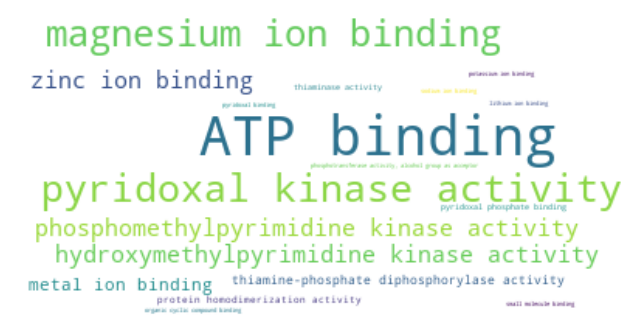
\includegraphics[scale=0.35]{report/img/word_cloud_mf.png} \\
    \small{Molecular Function Terms}
\end{center}

\begin{center}
    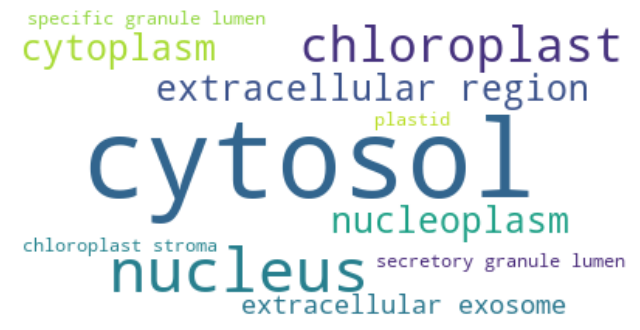
\includegraphics[scale=0.35]{report/img/word_cloud_cc.png} \\
    \small{Cellular Component Terms}
\end{center}

\begin{center}
    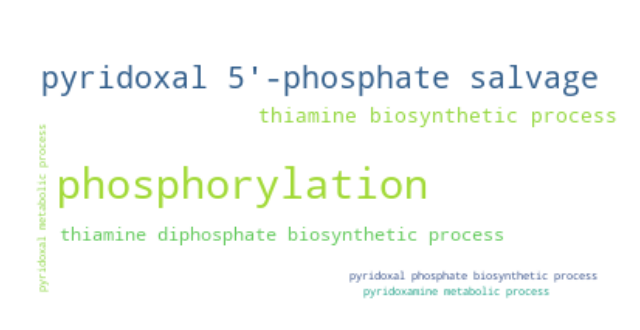
\includegraphics[scale=0.35]{report/img/word_cloud_bp.png} \\
    \small{Biological Process Terms}
\end{center} \\

Most enriched branches:\\



\subsection{Motifs}
Motifs are short protein sequences that are often repeated across the genome. These motifs usually coordinates protein-to-protein interaction and are found in the disordered regions. 

Our objective is to see if any commonly occurring linear motifs appear in our \texttt{PF08543} protein family and to do so we have at our disposal 2 datasets: ELM and ProSite.

For each member of the family we checked if the regular expressions found in the aforementioned 2 datasets were sub-sequences of it. However the vast majority of the matches found are outside of disordered regions (which can be found with the MobiDB-lite database). This is due to the fact that our protein family is constituted by globular proteins.

Given a motif, the regions where its pattern matches our proteins are overlayed onto multiple sequence alignments. These patterns are then visually inspected to determine the significance of pattern in the family.
Some patterns are overly general, matching many regions and are labeled as having a high probability of being observed in any given protein sequence from our family. (Example is the first plot)

Conservation of a pattern in the same position is indicative of functional significance.

\subsubsection{ELM}

There were 18 significant hits in this database
(Add the function of both of these motifs)

\begin{center}
    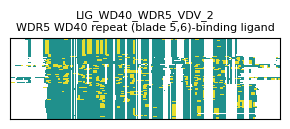
\includegraphics[scale=1]{report/img/Elm.png} \\
    \small{Most common Elm motifs in our family}
\end{center}

% \begin{center}
    % \includegraphics[scale=0.4]{report/img/Elm2.png} \\
    % \small{10nth to 18nth most common ELM linear motifs}
% \end{center}

\subsubsection{ProSite}

There were 4 significant hits in this database:

\begin{center}
    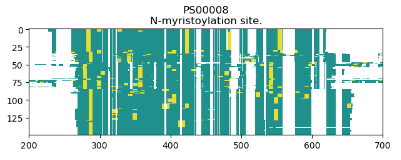
\includegraphics[scale=1]{report/img/prosite.png} \\
    \small{Most common ProSite motif in our family}
\end{center}


\section{Results}

\section{Discussion}




%-------------------------------------------------------------------------
\section{References}

List and number all bibliographical references in 9-point Times,
single-spaced, at the end of your paper. When referenced in the text,
enclose the citation number in square brackets, for
example.  Where appropriate, include the name(s) of
editors of referenced books.

%{\small
%\bibliographystyle{ieee_fullname}
%\bibliography{egbib}
%}

\clearpage % Start a new page
\onecolumn % Switch to one-column layout

\section{Appendix}


\subsection{Taxonomic Tree}
\label{sec:taxtree}

Below, we plot the full-resolution Taxonomic Tree. \\
\begin{center}
    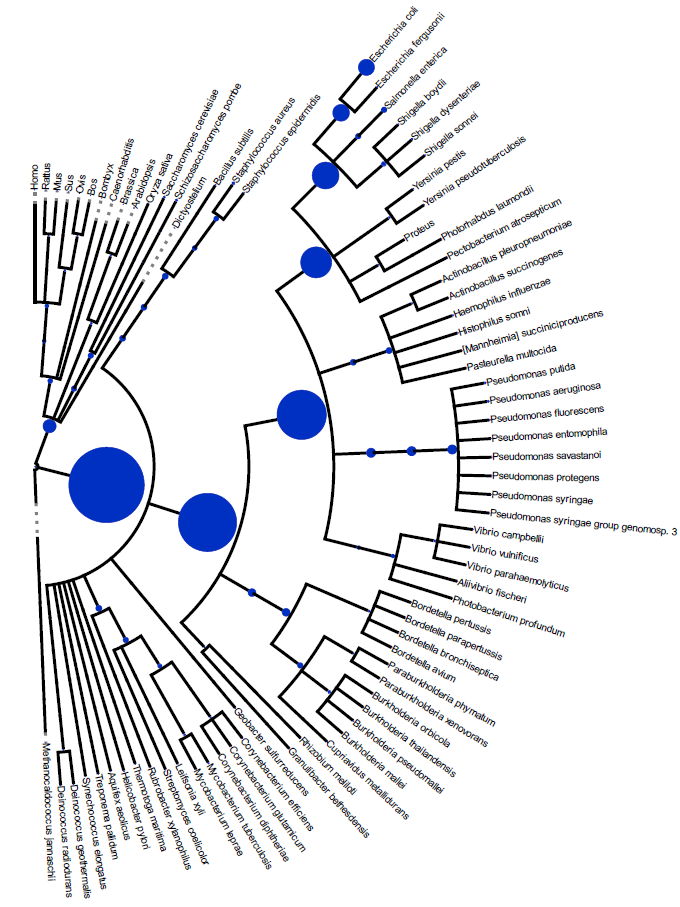
\includegraphics[]{report/img/taxonomy_tree.png}
\end{center}

\subsection{ELM}
\begin{center}
    \includegraphics[scale=0.4]{report/img/Elm1.png} \\
    \small{Top 9 most common ELM linear motifs}
\end{center}
\begin{center}
    \includegraphics[scale=0.4]{report/img/Elm2.png} \\
    \small{10nth to 18nth most common ELM linear motifs}
\end{center}

\subsection{ProSite}
\begin{center}
    \includegraphics[scale=0.4]{report/img/Prosite.png} \\
    \small{Most common 4 ProSite linear motifs}
\end{center}
\end{document}
